\documentclass{article}

\usepackage{minted}
\usepackage{amsmath}
\usepackage{amssymb}
\usepackage{enumitem}
\usepackage{fontspec}
\usepackage[margin=0.75in]{geometry}
\usepackage{longtable}
\usepackage{booktabs}
\usepackage{graphicx}
\usepackage{wrapfig}

\setmonofont{Fira Code}
\setminted{autogobble}

\title{Project M - Report}
\author{Adam Nicholls, George Chichirim, James Hobson, \\ Mihail Denkovski and Minh Le Quoc}

\begin{document}
\maketitle
We shall start by quoting our project brief as given to us.
\begin{quote}
  \textbf{Project M: Put your phone to work}

When people browse social media sites on their phones for hours every day, most of the CPU power goes unused. The old desktop equivalent of this problem was the screensaver, which did little of value until it was co-opted for distributed computing projects such as SETI@home. Your task is to make a platform that can perform useful computation in the background on a large number of mobile phones, while the owners are on social media - or even while they are asleep. It will have to run cross-platform, perhaps using JavaScript, but must also give the appropriate incentives to users - will it drain batteries or incur network charges? If so, what kind of application would customers pay to run on such a platform? Would phone sensors offer any specific value? You need to demonstrate an end-to-end solution including servers, mobile clients and an example application, keeping in mind the security implications if either customers or phone owners try to cheat the system.

[Project in collaboration with G-Research]
\end{quote}
The purpose of this document is to provide documentation, on building and usage of our code, as well as report on how the
code works and our individual contributions, as well as any ethical issues that may arise by the usage of this app.
\tableofcontents
\section{Usage}
The project is split into two parts, the first is the server and the second is the mobile app. Currently there is no way
to build the app for iOS, however a port is in progress so this is subject to change.
\subsection{Building}
The following instructions assume that you are building on a UNIX-Like system and have the following dependencies installed:
\begin{itemize}
  \item{Qt (Tested on version \(\geq 5.12.1\))}
  \item{autoconf}
  \item{Android SDK}
  \item{Android NDK}
  \item{JDK (or openJDK) version \(\geq 8\)}
  \item{GHC}
  \item{Cabal}
\end{itemize}
Autoconf is always needed, the final two dependencies are the server and the rest are for the app. All the additional haskell dependencies are installed
automatically when the \texttt{--enable-autodep} argument is passed to the \texttt{./configure} file.

Build instructions:
\begin{enumerate}
  \item{Clone the git repository \mintinline{bash}{git clone https://github.com/yobson/project-m && cd project-m}}
  \item{Build config files with the \mintinline{bash}{autoconf} command}
  \item{We then configure the program \mintinline{bash}{./configure} command with the following settings:
\begin{longtable}[]{@{}ll@{}}
\toprule
Option & Use\tabularnewline
\midrule
\endhead
\texttt{-\/-disable-app} & Don't build app\tabularnewline
\texttt{-\/-disbale-server} & Don't build server\tabularnewline
\texttt{-\/-enable-autodep} & Automatically install haskell
dependencies\tabularnewline
\texttt{-\/-with-qt-path=\textless{}path\textgreater{}} & Path to Qt
installation. You will probably want to set this\tabularnewline
\texttt{-\/-with-arch=\textless{}arch\textgreater{}} & Set android build
architecture. Options are: arm64\_v8a, armv7, x86\tabularnewline
\texttt{-\/-with-qt-version=\textless{}version\textgreater{}} & Set Qt
version. If not set, will choose newest version installed\tabularnewline
\texttt{-\/-with-live-address=\textless{}web\ address\textgreater{}} &
  Sets server address for app. f unset, will default to the test server \\ & address\tabularnewline
\texttt{-\/-with-projects-list=\textless{}path\textgreater{}} & Set ProjectM
server configuration file path.\tabularnewline
\bottomrule
\end{longtable}
    }
  \item{If all has worked, \mintinline{bash}{make -j} will build the app (\texttt{-j} enables parallel jobs) and produce a 
    file named \texttt{ProjectM.apk} which can be installed on an android phone.}
\end{enumerate}
If for any reason these instructions do not work (or you are trying to build for iOS), open the \texttt{.pro} file in QtCreator.
\newpage
\begin{wrapfigure}[38]{r}{0.5\textwidth}
  \centering
  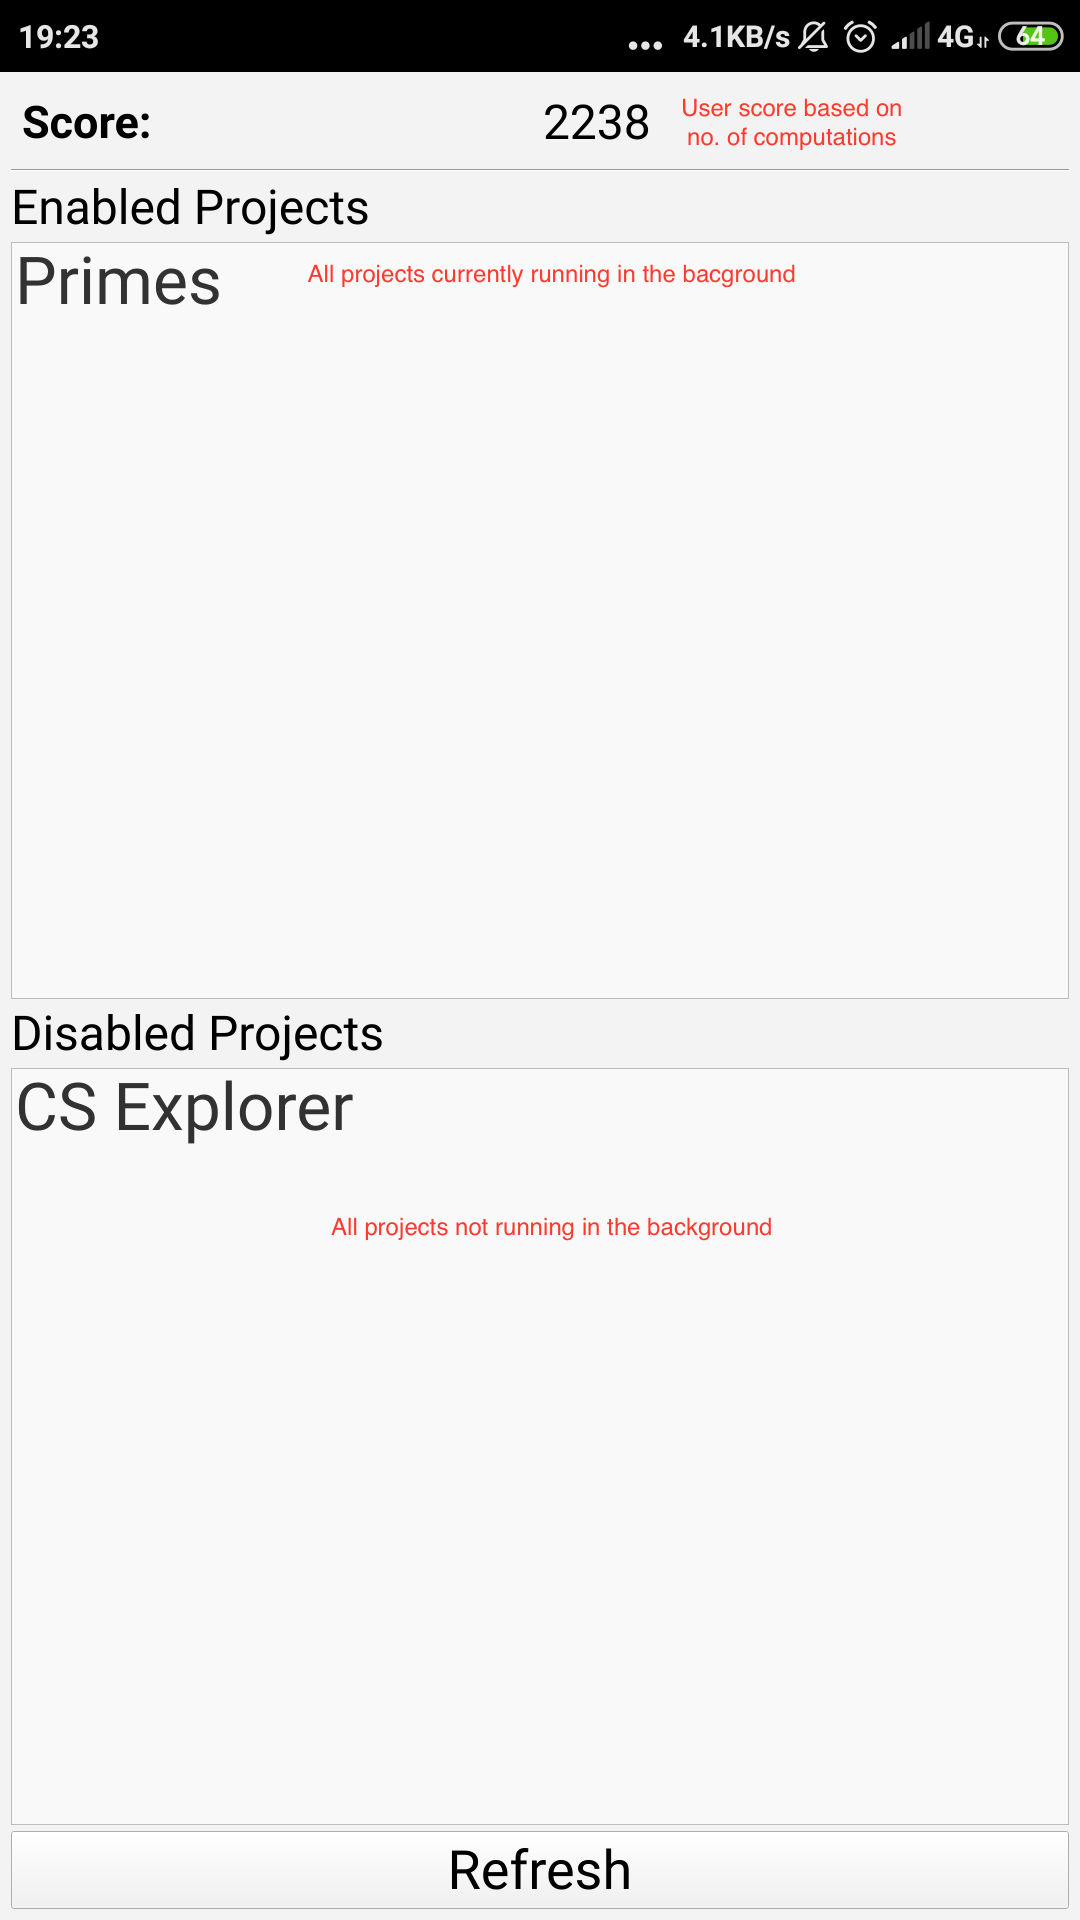
\includegraphics[width=0.5\textwidth]{DocFiles/main_page}
  \caption{Main app page}
\end{wrapfigure}
\subsection{Using the App}
When you launch the app for the first time, you will be prompted for your first and last name. There is no need for a password because
no user data is stored in the server (other than name-id pairs).
When the app is reopened and after registration, the user is greeted with their score and lists of projects. Figure 1 shows 
the main page with the red text explaining what they mean.

Clicking on each project will bring up a new page where you can chose weather to enable or disable each project, decide the 
rate in which the project will run a task (normally between once every 30 second to every 10 minutes). When you enable
a project, if permissions such as location are required, the user will be prompted to choose weather they really want to
enable the project. There is no way that the app can use permissions without the users consent.

\subsection{Configuring the Server}
If you want to host a ProjectM server, their are 3 things you have to consider:
\begin{enumerate}
  \item{Web server software - we use apache for the live server and lighttpt in production but any server with CGI will do e.g. NGINX}
  \item{A place to store the ProjectM Project list - the default is in the tmp directory\dots you really don't want to keep it here!}
  \item{Making sure apps are directed to the right place - the default is \texttt{www.hobson.space}}
\end{enumerate}

Firstly, setting up the server is easy. As long as the \texttt{.cgi} files are in the appropriate place with respect
to your webserver software of choice, for example, in our setup (FreeBSD \& Apache), all of the compiled server files and
projects live in \texttt{/usr/local/www/apache24/cgi-bin/}. It must be the case that all of the \texttt{.cgi} files can 
\textit{accsessed} from a web address in the following format `\texttt{base-addr.something/cgi-bin/*.cgi}' Make sure redis is installed!

The ProjectM configuration file is a text file that lists all of the projects in Haskell tuple format.
Here is an example file:
\begin{minted}{haskell}
  ("Project 1", "Description", "project1.cgi")
  ("Project 2", "Description", "project2.cgi")
\end{minted}
You can store this file where ever you like, but you need to specify the location in the configure file with the \texttt{--with-projects-list}

The base address that the mobile app uses is hardcoded for security reasons. This, just like the project list file, also has to specified when building
the app with the \texttt{--with-live-address} option.

\newpage
\subsection{Writing New Projects}
I shall explain how to write a new project with an example.
\begin{minted}{haskell}
import ProjectM

type State = (Integer, Integer, Int) -- Largest, Last Checked, ID of largest

jsMin = "(function(id, number){var n = parseInt(number);"
     ++ "for (var i = 2; i <= Math.sqrt(n); i++)"
     ++ "{if (n % i == 0){return id + \" \" + 0}}"
     ++ "return id + \" \" + n;})"

genPage :: Integer -> Int -> String
genPage prime id = concat ["<head><meta http-equiv=\"refresh\" content=\"30\">",
  "</head><body><h2>Largest prime found is ", show prime, "</h2>",
  "<h3 id=\"finder\">Finder: ", show id,
  "</h3></body>"]

nextOdd :: (Integral i) => i -> i -> i
nextOdd p i | i < p          = p + 2
            | i `mod` 2 == 0 = i + 1
            | otherwise      = i + 2

updater :: Updater State Integer
updater state             RequestJS      = (state, Send jsMin)
updater state@(lg,ch,id)  RequestInput   = ((lg,nextOdd lg ch ,id), 
                                           Send $ show (nextOdd lg ch))
updater state@(lg,ch,id) (ReturnAns n i) | i > lg    = ((i,ch,n), Yeet)
                                         | otherwise = (state, Yeet) 
updater state@(lg,ch,id)  ShowProject    = (state, Send $ genPage lg id)
updater state             RequestPermissions = (state, formatPermissions [])

main = runSite "primes" updater (2,2,1000)
\end{minted}
The general idea is that there is a (user defined) state data type. As the project runs, the project is fed events which
are used to update the state and return input to the phone.
\begin{itemize}
  \item{All ProjectM projects must import \texttt{ProjectM}}
  \item{The \texttt{State} type we define encodes the state at any given point. It must be readable and showable!}
  \item{\texttt{jsMin} is the javascript that is sent to the phone. It is given two string inputs, the first is the user ID and the second is
    a string specified by the server as input (we shall get to that later). This one is a function that checks to see if a number is prime.}
  \item{\texttt{genPage} is an auxiliary function we defined to generate the display page.}
  \item{\texttt{nextOdd} is a function defined to find the next number to check}
  \item{\texttt{updater} is a function that takes a state, event, and returns a tutple, \texttt{(next state, what to return to phone).} You \textbf{must} 
    define this function on all options. The type is \texttt{Updater a b} where \texttt{a} is the state type and \texttt{b} is the type that the phone returns.}
  \item{\texttt{main} function calls \texttt{runSite}. This gets a unique identification string (for DB reasons), the update function and an initial state.}
  \item{This app requires no permissions, but if it did, you would add them to the permissions list (passed to \texttt{formatPermissions}). Currently the only permission
    option is \texttt{Location}.}
\end{itemize}

\section{Project Structure}
The execution of this task is most certainly open to interpretation and fortunately we had the freedom to choose whichever
approach we deemed appropriate given the time restraints. In this section I will outline the general structure of the project as well
as what our aims were when designing. Figure  is a UML(ish) diagram showing all of the different parts of our app.
\begin{figure}[h]
  \caption{Diagram describing the structure of the project}
  \centering
  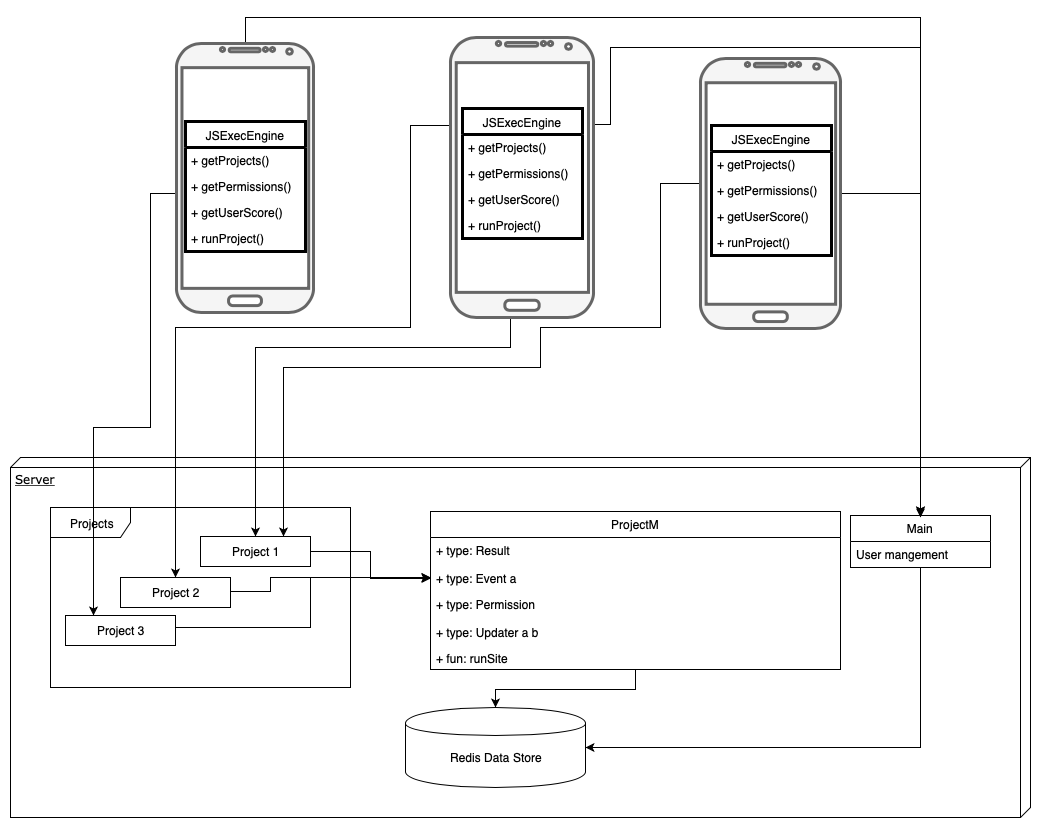
\includegraphics[width=1\textwidth]{DocFiles/ProjectM}
\end{figure}

The server is split into 3 parts: 
\begin{itemize}
  \item{The redis database - not made by us but chosen for high speed and small memory footprint} 
  \item{The main server, used for user management} 
  \item{The projects that make use of the ProjectM library for all access to the phones and resources}
\end{itemize}
All parts of the server are written in Haskell and CGI. Haskell was chosen because it is aggressively type safe and immutability reduces the
chance of obscure runtime errors. As a result, all parts of the server have been running since the first test without a single error! It
was also chosen for the \texttt{ProjectM} library because we wanted to ensure that all of the projects, whoever they are written by,
are up to similar standards of stability. Haskell is a compiled and efficient programming language meaning each project consumed very little space
and many projects can run simultaneously without slowing the server too much. CGI was chosen because we wanted it such that if one app crashed, no others would.
Although there are more modern ways to achieve this, CGI had the advantage of adding negligible size to server binaries and
allows us to add projects and modify existing projects without affecting any of the other projects running.

The mobile app is made up of the following parts:
\begin{itemize}
  \item{Javascript Execution Engine - Deals with all communication between the phone and the server.}
  \item{GUI - The display of the app}
  \item{Background Service - The scheduler and executer of tasks}
\end{itemize}
The app was constructed in C++ using the Qt library. This was chosen because it is cross-platform, allowing us with little additional effort, compile for
every platform. On top of this, with the knowledge that this app was to be running full time in the background of the user's phone, it was crucial to
ensure a little memory and CPU was used as possible, this gives C++ a major advantage over any other cross-platform options as they are almost always
predicated non-native frameworks such as web-technologies or the .net framework.
\section{Detailed Descriptions}
\subsection{Server}
\subsubsection{User Management}
\subsubsection{Project Managment and Hosting}
\subsection{Mobile App}
\subsubsection{Service}
\subsubsection{Java Script Execution Engine}
\subsubsection{Graphical User Interface}
\section{Ethics}
\section{Group Member Contibutions}
\subsection{Adam Nicholls}
\subsection{George Chichirim}
\subsection{James Hobson}
\subsection{Mihail Denkovski}
\subsection{Minh Le Quoc}
\end{document}
